\chapter{Il potente e saggio Fabio Fazio nel magico mondo di LHC}
Forse, non tutti sanno che, Fabio Fazio, un po' come Britney Spears e i semiconduttori, \'e un grande appassionato di acceleratori e rivelatori di particelle al punto di possederne uno piccolino nei suoi appartamenti di Celle Ligure. Il Fazio \`e molto esperto e molto bravo a riconoscere i rivelatori faziosi da quelli utili come quelli a CERN. Come Dante scelse Virgilio per accompagnarlo nel suo viaggio attraverso l'aldil\`a io mi affido a lui affich\`e possa essermi guida e consiglio nel parlarvi di LHC e dell'esperimento ATLAS.

Now the serious part begins.

\lettrine{T}{his} analysis uses data collected during 2015 and 2016, coming from the ATLAS detector at LHC, as well as all simulations were performed in its context. It is a good thing to begin this work describing the main features of the LHC facility at CERN and giving an overviwew of the ATLAS experiment.

\section{The Large Hadron Collider}
Since the day of its starting up LHC became the most powerful accelerator, of any kind, in the world. It consists of a double ring of 27 kilometers lenght of superconducting magnets in which hadrons (protons or heavy ions) can be accelerates nearly up to the speed of light, or $\gamma\simeq7500$, and forced to collide in 4 specific points where the two rings intersects and likewise detectors take place.

After the Higgs Boson discovery there are many open questions in physics that LHC is trying to give an answer. Up to now, the main target of this project are:
\begin{description}
\item[Supersymmetric discoveries] Despite the Standar Model of particle physics (SM) is a well established theory it doesn't provide a theory for gravitation similar to those for the other forces. A hint might come from supesymmetry (SUSY) that hypothesises more massive particle than the ones we already know.
\item[Dark matter] Cosmological and astrophysical observations have shown that all visible matter accounts only for about 5\% of the mass/energy of the Universe. There are many experiment which tries to understand the nature of potential dark matter.
\item[SM particle property] A lot of properties of already known SM particle have to be defined with more precision. Since the production rate of \Wboson and \Zboson is high it is quite easy to verify any sort of deviation from SM predictions from this measurement and find prediction of new physics.
\item[Antimatter puzzle] LHC will also helps to investigate the matter/antimatter ratio. Even if after the Big Bang they have been produced in equal amount there is no explanation on why, as best of our knowledge, matter dominates the universe
\item[Quark-gluon plasma] Heavy ion collision at high energy, in which temperature can exceed the center of the Sun, can produce a state of plasma in which quarks are free. In this state detectors can study how the matter we know, in form of protons and neutrons in which confinement of quarks took place, has formed.
\end{description}

The most frequent collisions at LHC happen between protons. Before getting into the double ring they come across several machines which provide the first step of acceleration.

Protons are obtained from ionuzed hydrogen atoms and accelerated by Linac2 up to \SI{50}{MeV}, then injected into the Proton Synchrotron Booster (PSB), which accelerates them to 1.4 \GeV. Then the beam travels into the Proton Synchrotron (PS), where is pushed towards 25 \GeV, and into the Super Proton Synchrotron (SPS),  the second largest machine among all CERN's complexes consisting of a ring of 1.1 km radius, that speed the protons up to 450 \GeV, which is the minimum at which the LHC can maintain a stable beam. The main advantage in using protons instead of electrons and positron, as it was used to in LEP at CERN before LHC, is thanks to their higher mass that they reduce syncrotron radiation while being accelerated. Protons are delivered in bunches: each bunch contains \SI{e11} of them and every proton beam has 2808 bunches.

As mentioned earlier the LHC accelerator consists in a double ring complex of nearly \SI{27}{km} lenght. It is made up of 8 arcs containing the dipole bending magnets and 8 insertion consisting of a long straight section plus two transition regions. The purpose of the magnets, made of superconducting material such as Niobium-titanium or Niobium-tin (\ce{Nb_3Sn}), is to provide to the beam a stable orbit: dipole magnets keep the particles in an almost circular orbit (even when it is bent by the Moon) and quadrupole magnets focus the beam. There is a third type of magnet used before making a collision to enhance its probability. Acceleration is provided by radiofrequency resonant cavities which also keep the beam at a constant energy compensating for energy losses and distribute the protons in bunches. so that every bunch is divided by \SI{25}{ns} from another. LHC uses 8 cavities per beam each delivering \SI{5}{MV/m} at \SI{400}{MHz} giving the beam \SI{500}{keV} every turn. The cavities operate at \SI{4.5}{K} while magnets are kept at \SI{1.9}{K} by superfluid helium providing a magnetic field of \SI{8}{T}.
In order to to avoid collision between hadrons and gas particles in the tubes, vacuum has to be made in them down to a pressure of \SI{e-13}{atm}.

The LHC was designed to operate with a \cm energy of $\sqrt{s}=\SI{14}{TeV} $ for protons, even if this energy has never been reached yet, and \SI{1150}{TeV} (or \SI{5.12}{TeV/u}) for heavy ions, and a rate of collision of \SI{e34}{cm^{-2}.s^{-1}} express in term of instantaneous luminosity. 

In LHC the insantaneous luminosity is computed via the formula:
\begin{equation}
	L=\frac{f_{\textup{LHC}} \cdot n \cdot N_{\textup{bunch}}^2}{A}
\end{equation}

where $f_{\textup{LHC}}$ is the collision frequency, $n$ is the number of bunch colliding, $N_{\textup{bunch}}$ is the number of particle per bunch and $A$ is inverse cross section of bunches. Instantaneous luminosity can be increas for example by reducing the bunch section or increasing the number of protons per bunch.

With the instantaneous luminosity one can forsee the number of event expected after a collision. Since the event rate is given by $\Gamma=\mathcal{L}\times\sigma$, where $\sigma$ is the total \pp cross section which at $\sqrt{s}=\SI{13}{Tev}$ is about \SI{80}{mb}, we expect a rate of about \SI{e9}{s^{-1}}. Along with istantaneous luminosity an integrated luminosity is defined by simply integrating on time both members of the previous equation, in formul\ae:
\begin{gather}
	L=\int{\mathcal{L}dt} \notag\\
	N=L\times\sigma
\end{gather} 

Among this events one can distinguish \emph{soft collisions} and \emph{hard collisions}.
\begin{description}
\item[Soft collisions]
\item[Hard collisions]
\end{description}

\begin{table}[tp]
	\centering
	\begin{tabular}{lc}
	\toprule
	Quantity& Amount\\
	\midrule
	Circumference& \SI{26659}{m}\\
	Dipole operating temperature& \SI{1.9}{K}\\
	Energy, protons& \SI{6.5}{TeV}\\
	Energy, heavy ions& \SI{2.56}{TeV/u}\\
	Peak magnetic dipole field& \SI{7.74}{T}\\
	Distance between bunches& $\sim$ \SI{7.5}{m}\\
	Peak Luminosity (protons)&  \SI{2.06e34}{cm^{-2}.s^{-1}}\\
	No. of bunches per proton beam& 2808\\
	No. of protons per bunch (at start)& \SI{1.2e11}{}\\
	Number of turns per second& \num{11245}\\
	Number of collision per second& $\sim$\SI{e6}{}\\
	
	\bottomrule
	\end{tabular}
	\caption{Table listing the main features of LHC}
\end{table}

\begin{figure}[tp]
	\centering
	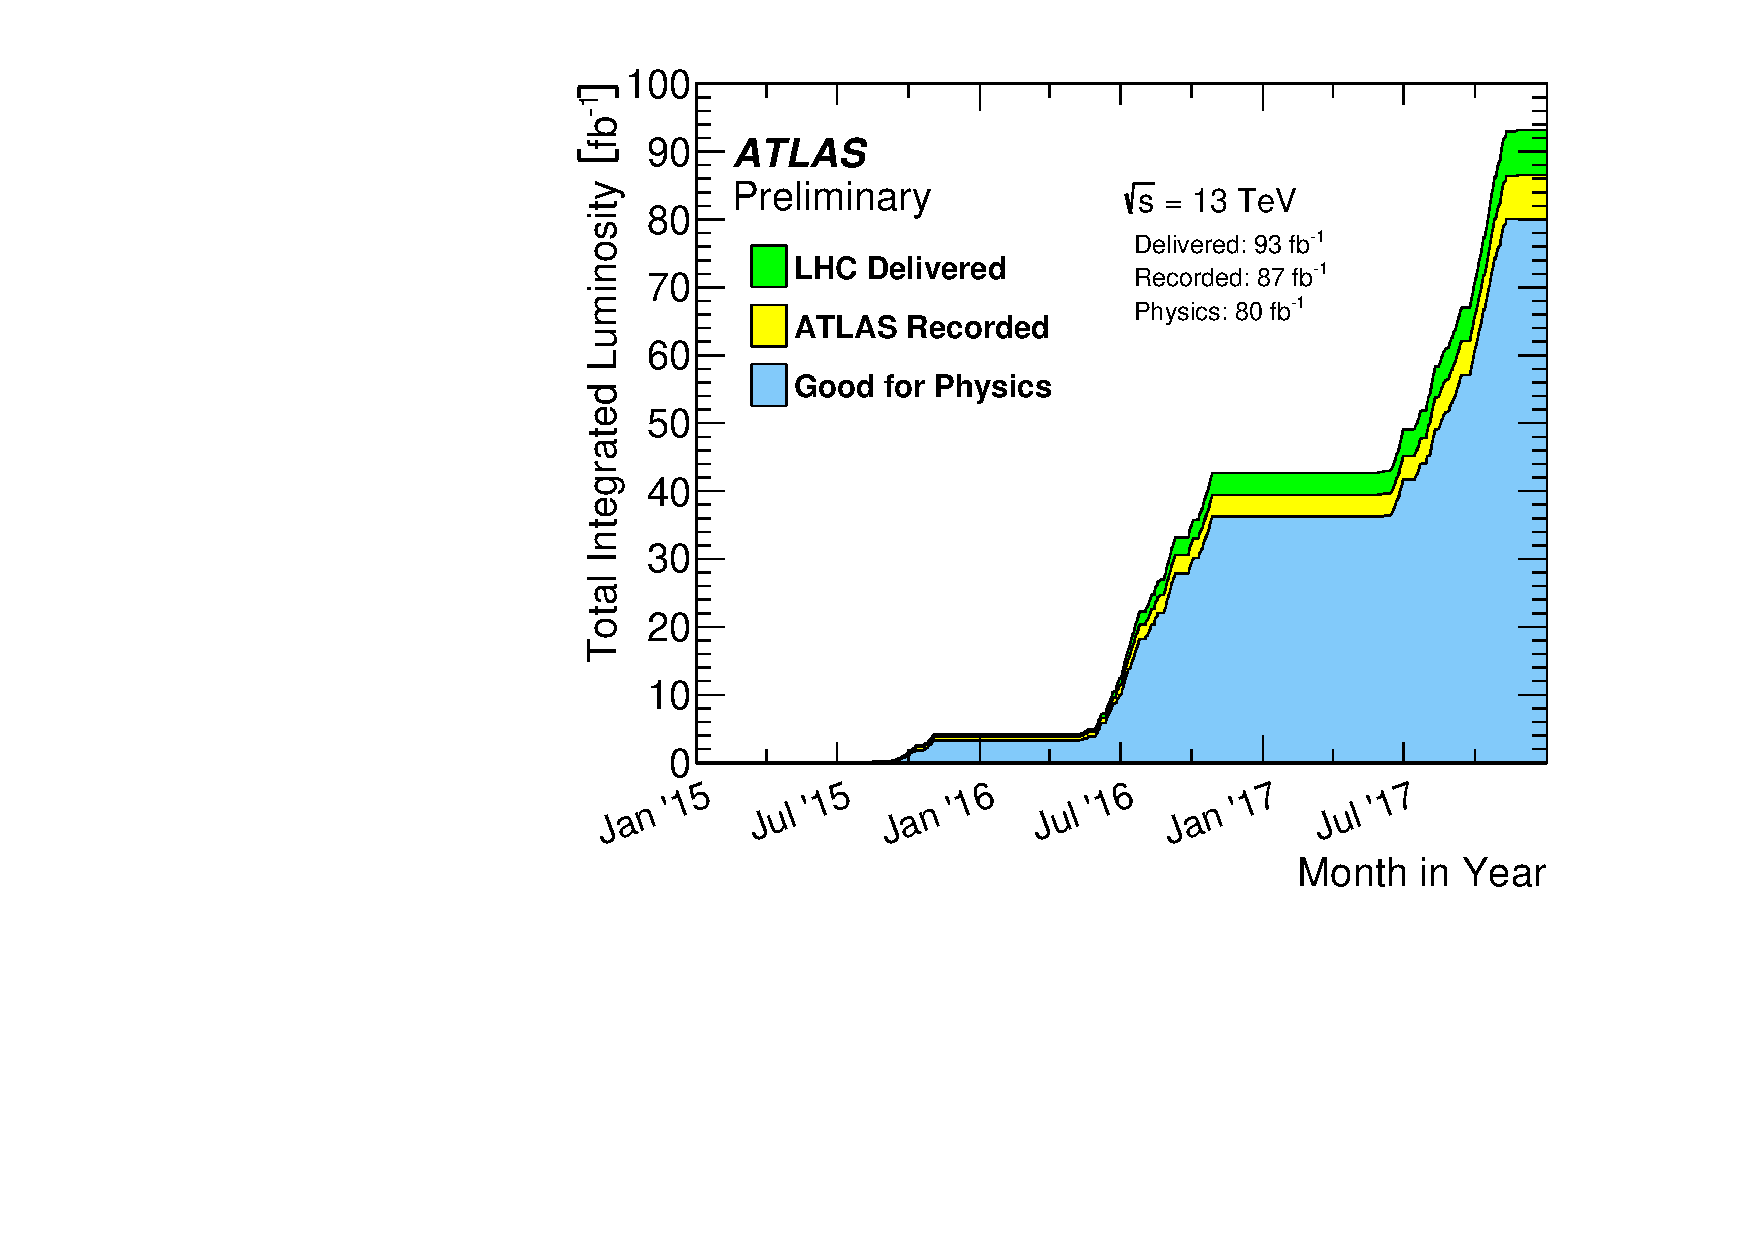
\includegraphics[width=0.75\textwidth]{LHC_ATLAS/intlumivstimeRun2DQ.pdf}
	\caption{Cumulative luminosity versus time delivered to ATLAS (green), recorded by ATLAS (yellow), and certified to be good quality data (blue) during stable beams for pp collisions at \SI{13}{TeV} \cm energy in 2015-2017.}
\end{figure}
\begin{figure}[tp]
	\centering
	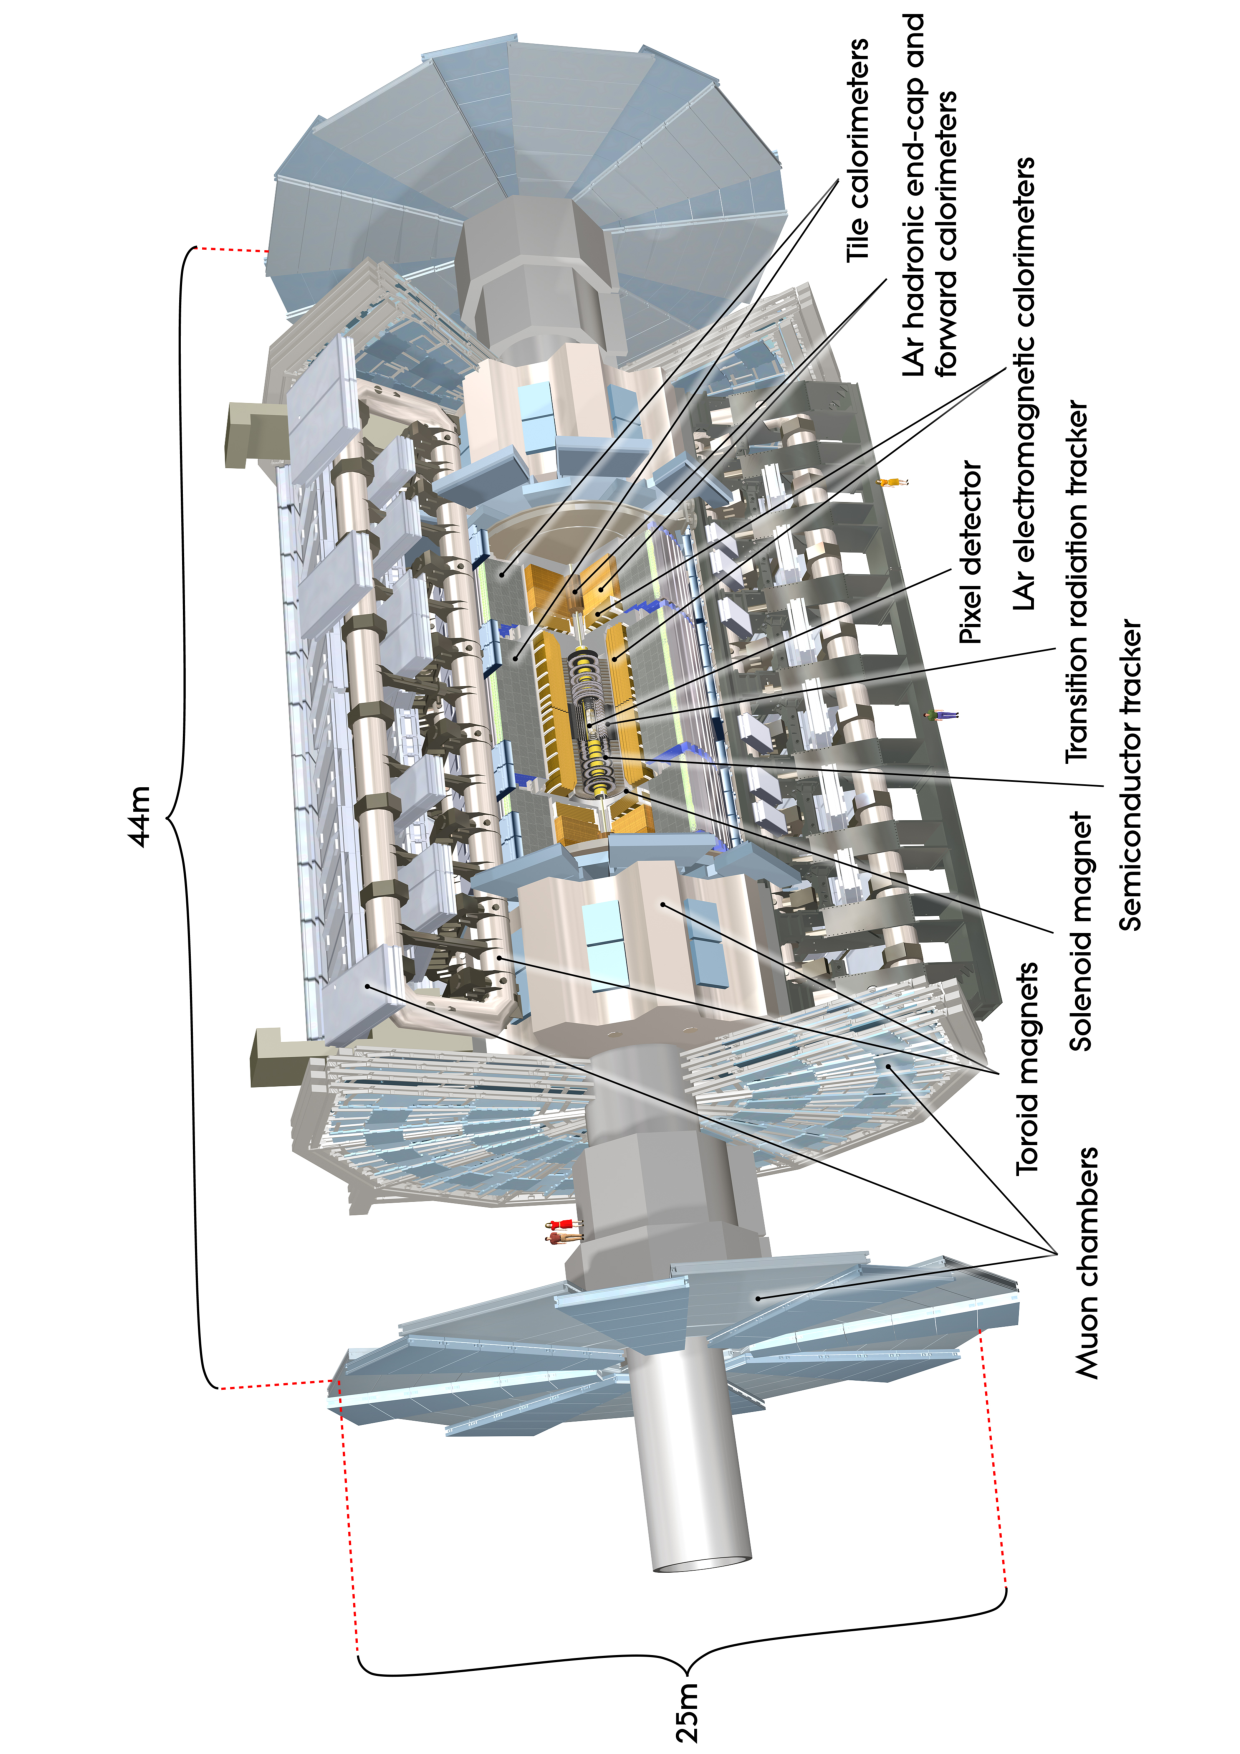
\includegraphics[width=0.75\textwidth]{LHC_ATLAS/0803012_01}
	\caption{TESTING}	
\end{figure}







